  \section{Conclusiones}

    % Para determinar la ecuación de cálculo del ángulo de desfasaje, a partir 
    % de la figura de Lissajous se debe tener en cuenta que

    % \begin{align*}
    %   f(t)=A \cdot sen(\omega \cdot t + \phi) \hspace{20pt} \land \hspace{20pt} g(t)=A \cdot sen(\omega \cdot t),
    % \end{align*}

    % donde g(t) es la señal de referencia, se coloca en el eje x de la figura por convención y
    % cada punto de la Figura de Lissajous se compone en coordenadas

    % \begin{align*}
    %  Lissajous(X,Y)= ( \hspace{5pt} g(t) \hspace{10pt} ; \hspace{10pt} f(t) \hspace{5pt}).
    % \end{align*}
    
    % Si se hace $t=0$, entonces $g(t)=0$, y 

    % \begin{align*}
    %   f(0)=A \cdot sen(\phi) \hspace{20pt} \Longrightarrow \hspace{20pt} \Aboxed{sen(\phi)=\frac{f(0)}{A}}.
    % \end{align*}

    % En la figura de Lissajous, f(0) se corresponde con el corte del trazo con el eje vertical, y A es el valor 
    % máximo absoluto que alcanza la señal.

    % Luego por trigonometría se puede deducir que:

    % \begin{align*}
    %   sen^2(\phi)+cos^2(\phi)=1 \hspace{20pt} \Longrightarrow \hspace{20pt} \Aboxed{cos(\phi)= \sqrt{1 +  \left( \dfrac{f(0)}{A} \right)^2} }.
    % \end{align*}

    %     \begin{figure}[H]
    %       \centering
    %         \frame{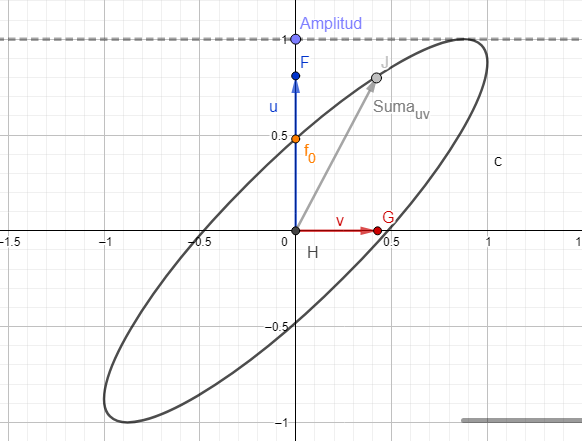
\includegraphics[width=0.7\textwidth]{Imagenes/Conclusiones/Figura_Lissajous_Geo.png}}
    %         \caption{Curva Lissajous.}
    %         \label{fig:Lissajous}
    %     \end{figure}

    % Para determinar la ecuación del cálculo del capacitor de compensación se parte de la siguiente
    % premisa:

    % \begin{align*}
    %   I_{Xc} = I \cdot sen(\phi) \hspace{20pt},
    % \end{align*}

    % donde $I_{Xc}$ es la corriente reactiva debido al capacitor, I la corriente total y $\phi$ el 
    % ángulo de desfasaje entre la tensión y corriente, el cual se quiere corregir.

    % Dividiendo ambos miembros por la tensión V total, se tiene

    % \begin{align*}
    %    \frac{I_{Xc}}{V} = \frac{I \cdot sen(\phi)}{V} \hspace{20pt},
    % \end{align*}

    % recordando además la ecuación de Reactancia de un capacitor que es

    % \begin{align*}
    %     Xc = \frac{V}{I_{Xc}} = \frac{1}{\omega \cdot C} \hspace{20pt},   
    % \end{align*}

    % se tiene entonces que

    % \begin{align*}
    %    \frac{1}{Xc} = \omega \cdot C = \frac{I \cdot sen(\phi)}{V} \hspace{20pt}.
    % \end{align*}

    % Usando la relación de potencia aparente se reemplaza I obteniéndose 

    % \begin{align*}
    %   \omega \cdot C = \frac{S \cdot sen(\phi)}{V^2} \hspace{20pt},
    % \end{align*}

    % por último multiplicando y dividiendo el segundo término por $cos(\phi)$ y despejando C

    % \begin{align*}
    %    \omega \cdot C = \frac{ \frac{S \cdot cos(\phi) \cdot sen(\phi)}{cos(\phi)}}{V^2}\hspace{20pt} \Longrightarrow \hspace{20pt} \Aboxed{C = \frac{P \cdot tg(\phi)}{\omega \cdot V^2}}\ .
    % \end{align*}

    Los métodos utilizados para medir el desfasaje de tensión y 
    corriente, se corresponden entre sí en los resultados, lo que da una idea de la fidelidad 
    de los mismos para la determinación de éste parámetro.

    Por otro lado, se ha visto en el desarrollo del presente informe que, debido que la red posee una composición 
    armónica, es decir no es senoidal pura. Debido a lo anterior, al conectar el capacitor se produce un realce de 
    las altas frecuencias, y el aporte en amplitud de los armónicos en la señal es 
    notorio. Como consecuencia de lo anterior expuesto, se observa una deformación en la señal de 
    salida debido a la influencia de dicho capacitor de compensación.

    Como complemento al experimento \ref{subsubsec:Medicion del factor de potencia corregido}, 
    donde se obtuvo la potencia aparente debido a la corrección del factor de potencia, se realiza un análisis en el 
    dominio del tiempo, empleando los filtros digitales del osciloscopio. El mismo permite dar un acercamiento 
    al nuevo desfasaje ya que, como se ha mencionado en dicha sección, mediante el modo X-Y se complica 
    determinarlo. La Figura \ref{fig: Desfasaje tensión-corriente.} muestra la nueva señal filtrada, 
    con ésta puede procederse a realizar un cálculo en relación a la proporcionalidad entre pulsación 
    angular y tiempo, y de ésta manera obtener el nuevo desfase.

    % Adicionalmente, puede determinarse el factor de potencia corregido, a partir de las señales
    % obtenidas en el tiempo. El principal problema es la cantidad de armónicos montados sobre 
    % la señal de corriente, para resolverlo se debe aplicar un filtro pasa bajos a la misma, de
    % ésta manera, es más sencillo realizar los cálculos.

        \begin{figure}[H]
          \centering
          \frame{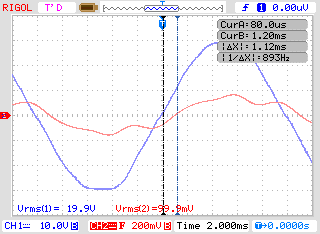
\includegraphics[width=0.45\textwidth]{Imagenes/ActividadPractica/CorreccionDeFdP/Exp2_15_Vin-Iin-ConCapacitorYFiltroEnOsc.png}}
          \caption{Medición del desfasaje de tensión y corriente usando filtros.}
          \label{fig: Desfasaje tensión-corriente.}
        \end{figure}      

    


    

    
